\documentclass{article}
\usepackage{amsmath,amssymb,amsbsy,amsfonts,amsthm}
\usepackage{graphics,epsfig,graphicx,float,subfigure,color}

\title{Literature Review}
\author{Abraham Frei-Pearson \\
	Department of Mathematics  \\
	\and 
	Sheroze Sheriffdeen \\
	Oden Institute \\
	}

\date{\today}
% Hint: \title{what ever}, \author{who care} and \date{when ever} could stand 
% before or after the \begin{document} command 
% BUT the \maketitle command MUST come AFTER the \begin{document} command! 
\begin{document}

\maketitle

\section{Proposal}

{\em This section is unaltered from our proposal, including a few typos; we include it for reference.}

We are interested in applying reinforcement learning techniques to noisy optimal control problems. The general case will be in the following form. Given an unknown $n \times n$ matrix valued function $A$, our state will be a vector $x_t \in \mathbb R^n$, and our dynamics will be
\[
    x_{t+1} = (I + A(x_t)) x_t + u(x_t) + g,
\]
where $g$ is Gaussian noise. Here $u$ will be a control function, which we are trying to learn, which will be specified in different problem domains. In general, we'll take $u$ to be bounded. We could consider the avoid problem: we would like $x$ to avoid a certain region. We could also consider the reach problem: we would like $x$ to reach a specified neighborhood of the origin (say) in time as small as possible.

Cartpole, or inverted pendulum, is a basic example of this sort of problem in the noise free setting, and it will be our starting point. To start with we'll consider {\em bang-bang} controls only: the cart can be accelerated either left or right with full force at each time. With this in mind, the problem admits the following description:
\begin{enumerate}
    \item []{\em State space}: This is the position of the cart, and the angle and angular velocity of the pendulum, so it is $\mathbb R \times (0,\pi) \times \mathbb R$.
    \item []{\em Action space}: This is just whether we are accelerating the box left or right, so $\{\pm 1\}$.
    \item []{\em Reward function}: We will take this to be $-1$ if the pendulum falls past a given threshold, and $0$ otherwise.
\end{enumerate}

In the noise-free setting, the inverted pendulum is stable with an appropriate control. On the other hand, if the noise term is large enough compared to the size of the control, the pendulum will tip over quickly no matter what you do. It would be interesting to compute this relationship empirically and see how common reinforcement learning algorithms compare.
We will also explore the same problem in the noise-free setting with noisy observations. In this case, the state should include previous observations, since these can be used to more appropriately approximate the true state of the system.
If this goes well, we would like to explore some of the other optimal control problems in the OpenAI gym.

There are a number of reach goals which would be of interest. What if damping is added to the inverted pendulum, i.e. the acceleration caused by the control depends on the position of the cart. This problem is interesting in the one-shot case: suppose the dynamics (i.e. the matrix $A$ above) is chosen randomly. What is the best strategy for computing $u$? In this case, we will need to move away from bang-bang controls: it makes sense to hold off on firing the control, or fire it at a small velocity, early on to learn the system dynamics. Could the reach or avoid problems be solved safely in this case?

There are several abstractions we are interested in considering: noise in the system itself, noise in the observations, and noise in the reward. In what follows, we will refer to a problem as "traditional optimal control" if the noise-free dynamics are known, and "reinforcement learning" if they are not. 

Noisy dynamics introduce maximization bias, as discussed in Sutton and Barto ~\cite{suttonAndBarto}, into the standard reinforcement learning algorithms. The point is that, early in training, noise causes the best-looking action to look better than it actually is. This is dealt with effectively by double-Q learning. Another algorithm for dealing with maximization bias is discussed in \cite{foxPakmanTishby}, so called "G-learning". This algorithm begins with a stochastic policy $\rho$. A pseudo-reward is calculated for each state action pair called $G_\pi(s,a)$, where $G_\pi(s,a)$ is $Q(s,a)$ less an information cost which is a discounted version of the Kullback-Liebler divergence $KL(\pi( \dot , s) || \rho( \dot , s))$.

In the case of traditional optimal control, at least when the state dynamics are locally linear, an  optimal estimate for the state is given by extended Kalman filtration ~\cite{welchBishop}. This is optimal in the sense that, given knowledge about the noise, the Kalman estimate for the state minimizes the expected squared error. The Kalman estimate is as follows: suppose the matrix $A$ above is known, and our estimate for $x_t$ is $\hat x_t$. We obtain an estimate for $x_{t+1}$ by applying $H := I+A$ to $\hat x_t$. If $z$ is the observed value at time $t+1$, then we set $\hat x_{t+1} = x_{t+1} + K (z - x_{t+1})$, where $K$ is the {\em Kalman gain}, obtained by minimizing the a posteriori variance of the estimate. We would like to see how much applying the Kalman filter to our data in a noisy environment improves the usual reinforcement learning methods. Although we need a model to apply the Kalman filter, it would still be interesting to study improvements to reinforcement learning from filtered data. Kalman filtration is also applied to reinforcement learning problems in ~\cite{trippSchacter} in a somewhat different way: in this case Kalman filtration is applied to the update of the $Q$-function directly, and then $Q$-learning is applied.

We are also interested, time permitting, in studying noisy problems in the one-shot case. Consider a discrete, linear dynamical system with noise
\[
    x_{t+1} = (I + A) x_t + \eta + u_t x_t,
\]
where $\eta$ is Gaussian and $u_t$ is a linear control. Our reward will be $1$ for all $t$ where $x_t$ is within a ball around the origin. What if the matrix $A$ is unknown a priori? This problem is studied in ~\cite{ornikIsraelTopcu} and \cite{ahmadiIsraelTopcu}, using the theory of differential inclusions. This is also addressed in ~\cite{bagnellNgSchneider} in the min-max setting. Given a set of transitions $\mathcal P$, an algorithm for producing a policy maximizing $\mathbb E_{p \in \mathcal P, \Pi} \sum\limits_t \gamma^t R(X_t)$, where $X_t$ is the trajectory under $\pi$, is presented. It would be interesting to see if this algorithm could be adjusted to include a prior on the transitions, and optimize the expected reward according to that prior rather than the min-max reward. We would be interested in studying some simple examples of this in the context of reinforcement learning, in simple tabular or one dimensional cases. 



A reformulation of the stochastic optimal control problem in terms of KL divergence minimization is examined by Rawlik et. al \cite{rawlik2013stochastic}. This work considers reinforcement learning as an instance of stochastic optimal control which does not assume knowledge of the dynamics.  A cost is associated with each policy relating to a measure of the control, and the stochastic optimal policy is posed as finding an optimal policy that minimizes the expected cost of controls following trajectories under the given policy. An experiment performed with the cart-pole problem with zero mean Gaussian noise added to the state and an extended Kalman smoother \cite{stengel1986stochastic} is use to estimate a Gaussian approximation to the full posterior of the state variables, leading to a Gaussian posterior policy.
\iffalse
A specific instance of stochastic optimal control is the reinforcement learning (RL) formalism  which does not assume knowledge of the dynamics or cost function, a situation that may often arise in practice.  Let $\mathcal{C}_t(x, u) \ge 0$ be the cost incurred per stage for choosing control $u$ in state $x$ at time $t$. The SOC problem consists of finding a policy which minimises the expected cost, i.e., solving
\begin{equation}
    \pi^* = \underset{\pi}{\mathrm{argmin}} \left \langle i  \sum_{t=0}^T \mathcal{C}_t (x_t, u_t) \right \rangle_{q_{\pi}}
\end{equation}
where $\langle \cdot \rangle_{q_{\pi}}$ denotes the expectation with respect to the distribution over trajectories under policy $\pi$.
\fi

\section{G learning}

\subsection{Description of the algorithm}

We begin by recalling the setup for $Q$-learning. For consistency with ~\cite{foxPakmanTishby}, we will state the algorithm in terms of costs rather than rewards. For an MDP with discount $\gamma$, a state-action value function $Q$, and an observed state, action, cost, and new state $s,a,c,s'$, we perform the update $Q(s,a)=\alpha Q(s,a) + (1-\alpha) (c + \gamma \arg \min\limits_{a'} Q(s',a))$. Action are chosen according to a policy which is $\epsilon$ greedy with respect to $Q$.

Although there are robust convergence guarantees for $Q$-learning, in the presence of noise $Q$-learning converges very slowly. The reason is this: suppose that, early in training, we observe a particularly low value of $Q(s,a)$ early in training due to stochasticity. Then, with high probability, the action $a$ will be chosen whenever the MDP is in the state $s$, preventing exploration.

$G$ learning is obtained from $Q$ learning by adding an information cost with respect to a given baseline policy $\rho$. Specifically, $g^\pi(s,a) = \log(\frac{\pi(a | s)}{\rho(a | s)})$. Then the information cost of a state $s$ is
\[
    I^\pi(s) = \sum\limits_{t \geq 0} \gamma^t \mathbb E [g^\pi(s_t,a_t) | s_0 = s].
\]
Set set the state value to be $F^\pi(s) = V^\pi(s) + \frac{1}{\beta} I^\pi(s)$. The number $\beta$ is a parameter which can be tuned to the problem and the baseline policy $\rho$. The state action function $G^\pi(s,a)$ is then defined as
\[
    G^\pi(s,a) = \mathbb E(c|s,a) + \gamma \mathbb E(F^\pi(s')|s,a],
\]
where $c$ is the cost and $F^\pi(s')$ is the state value of the next state. We thus obtain 
\[
    F^pi(s) = \sum\limits_{a} \pi(a|s) (\frac{1}{\beta} \log \frac{\pi(a|s)}{\rho(a|s)} + G^\pi(s,a).
\]
Setting the gradient of this with respect to $\pi(a|s)$ to zero gives
\[
    \pi(a|s) = \frac{\rho(a|s) e^{-\beta G(s,a)}}{\sum\limits_{a'} \rho(a'|s) e^{-\beta G(s,a')}}.
\]
This leads to the update
\[
    G(s,a) \leftarrow (1-\alpha) G(s,a) + \alpha(c - \frac{\gamma}{\beta} \log(\sum\limits_{a'} \rho(a'|s') e^{-\beta G(s',a')})
\]
given the observation $s,a,r,s'$.

The temperature parameter $\beta$ encodes how much preference is given to the prior policy $\rho$. When $\beta$ is small, $G$-learning heavily penalizes policies which are different from $\rho$. In the limit, when $\beta = 0$, $G$-learning will only allow the function $\rho$ to be used. On the other hand, as $\beta \to \infty$, the behavior of $G$-learning tends to that of $Q$-learning. In practice, we set $\beta = i$ for the $i$th episode.

\subsection{Experiment}

We tested the performing of $G$-learning against $Q$-learning in the simple gridworld setup of ~\cite{suttonAndBarto}, example 4.1. Here we have a 4x4 grid with terminal states in the upper left and lower right corners, with a reward of $-1$ (or a cost of $1$) for each transition. We trained a $Q$-learning and a $G$-learning agent on this environment: we ran trained 200 independent agents on $Q$- and $G$-learning each for 40 episodes, and recorded the cumulative score. We took the learning rate $\alpha$ to be $0.1$, the parameter $\epsilon$ in $Q$-learning (the $\epsilon$ with respect to which the policy is $\epsilon$-greedy) to be $0.1$, the prior policy to be uniform at random, and the temperature parameter $\beta$ to be $i$ in the $i$th episode. Note that in all cases $G$-learning outperforms $Q$-learning, but $G$-learning performs even better in the case of greater noise.

In the figure below, the $x$ axis represents the size of the noise term: for each $x$ we added a uniform random variable to the return drawn from $[-x,x]$. The $y$-axis represents the difference in the cumulative reward over the 40 episodes between $Q$-learning and $G$-learning, averaged over all 200 runs.

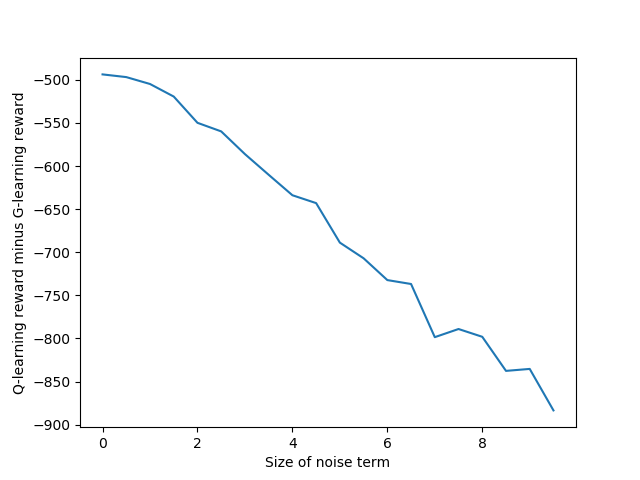
\includegraphics[]{noisevsreward.png}

\bibliographystyle{plain} 
\bibliography{references}

\end{document}
